\documentclass[12pt]{article}
\usepackage{hyperref}
\usepackage{graphicx}
\usepackage{caption}
\usepackage{geometry}
\usepackage{float}
\usepackage{amsmath}
\usepackage{algorithm}
\usepackage{algpseudocode}
\usepackage{tikz}
\usepackage{enumitem}
\usepackage{tabularx}
\usepackage{makecell}
\usepackage{biblatex}
\usepackage{appendix}
\usepackage{subcaption}
\usepackage{listings}
\usepackage{wrapfig}
\usepackage{ragged2e}
\usepackage{booktabs}
\usepackage{pgfplots}

\addbibresource{bibliography.bib}

\geometry{a4paper, margin=1.5cm}
\setlength{\parindent}{0em}
\setlength{\parskip}{0.5em}

\begin{document}

\begin{titlepage}
    \centering
    \vspace*{3cm}
    {\Huge\bfseries Deliverable exercise FC: Compound Pendulum\par}
    \vspace{1cm}
    {\large Mauro VÁZQUEZ CHAS, Dániel MÁCSAI \par}
    \vspace{4cm}
    {\large \textbf{Master in Artificial Intelligence}\par}
    
\includegraphics[width=0.5\textwidth]{Logo_UPC.png}\par\vspace{1cm}
    {\large \textbf{Planning and Approximate Reasoning}\\ Work 4\par}
    \vspace{1cm}
    {\large\bfseries 10th January 2024\par}
\end{titlepage}

\pagestyle{empty}

\newpage
\tableofcontents
\newpage

% Set page numbering    
\setcounter{page}{1}
\pagestyle{plain}

\section{Introduction}
\label{sec:introduction}

\section{Design of the Fuzzy Controller}
\label{sec:desig}

\subsection{Membership functions}

\begin{figure}[H]
    \centering
    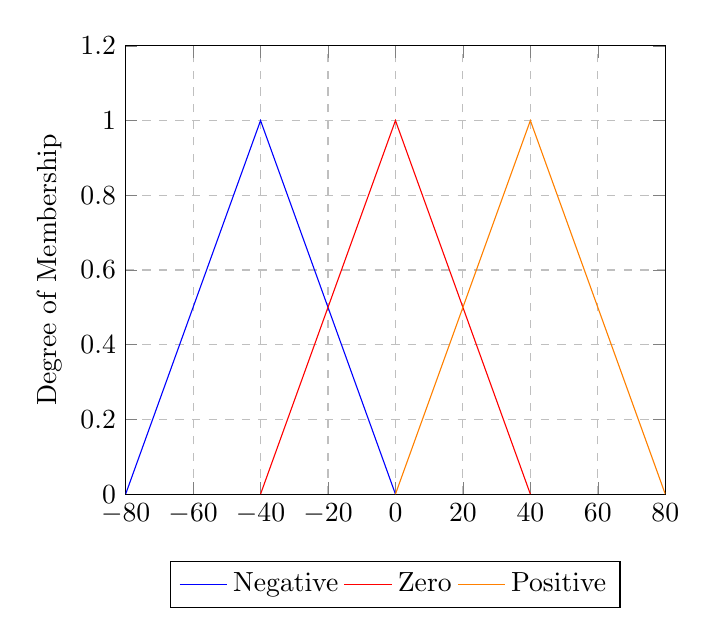
\begin{tikzpicture}
        \begin{axis}[
            ylabel={Degree of Membership},
            ymin=0, ymax=1.2,
            xmin=-80, xmax=80,
            legend style={at={(0.5,-0.15)},anchor=north,legend columns=-1},
            ymajorgrids=true,
            xmajorgrids=true,
            grid style=dashed
        ]
        
        % Negative Membership Function
        \addplot[solid, blue] coordinates {(-80,0) (-40,1) (0,0)};
        \addlegendentry{Negative}
        
        % Zero Membership Function
        \addplot[solid, red] coordinates {(-40,0) (0,1) (40,0)};
        \addlegendentry{Zero}
        
        % Positive Membership Function
        \addplot[solid, orange] coordinates {(0,0) (40,1) (80,0)};
        \addlegendentry{Positive}
        
        \end{axis}
    \end{tikzpicture}
    \caption{Membership Functions for Input Variable "Error"}
\end{figure}



\begin{figure}[H]
    \centering
    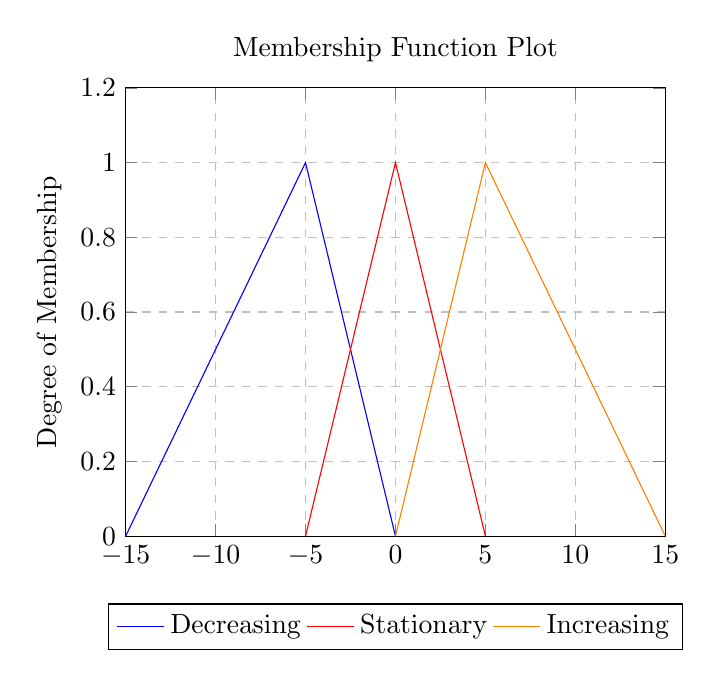
\begin{tikzpicture}
        \begin{axis}[
            title={Membership Function Plot},
            ylabel={Degree of Membership},
            ymin=0, ymax=1.2,
            xmin=-15, xmax=15,
            legend style={at={(0.5,-0.15)},anchor=north,legend columns=-1},
            ymajorgrids=true,
            xmajorgrids=true,
            grid style=dashed
        ]
        
        % Decreasing Membership Function
        \addplot[solid, blue] coordinates {(-15,0) (-5,1) (0,0)};
        \addlegendentry{Decreasing}
        
        % Stationary Membership Function
        \addplot[solid, red] coordinates {(-5,0) (0,1) (5,0)};
        \addlegendentry{Stationary}
        
        % Increasing Membership Function
        \addplot[solid, orange] coordinates {(0,0) (5,1) (15,0)};
        \addlegendentry{Increasing}
        
        \end{axis}
    \end{tikzpicture}
    \caption{Membership Functions for Input Variable "Error Derivative"}
\end{figure}

\textbf{Note:}
The range for the error derivative was modified from the initially proposed values of [-5, 5] to [-15, 15]. This adjustment was necessary because the original range was insufficient, causing the derivative to exceed its bounds. Consequently, the fuzzy controller outputted a value of zero during the Simulink simulation. The revised range provided more accurate and reasonable results.

\begin{figure}[H]
    \centering
    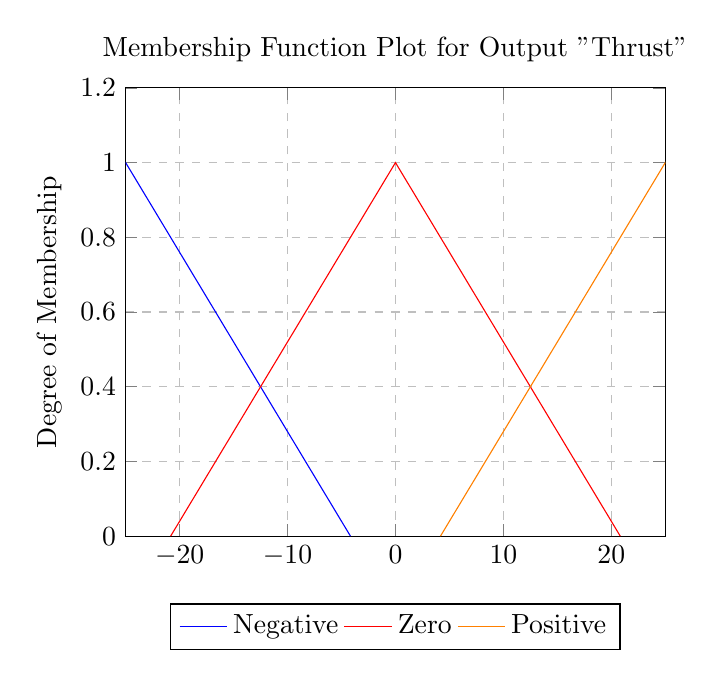
\begin{tikzpicture}
        \begin{axis}[
            title={Membership Function Plot for Output "Thrust"},
            ylabel={Degree of Membership},
            ymin=0, ymax=1.2,
            xmin=-25, xmax=25,
            legend style={at={(0.5,-0.15)},anchor=north,legend columns=-1},
            ymajorgrids=true,
            xmajorgrids=true,
            grid style=dashed
        ]
        
        % Negative Membership Function
        \addplot[solid, blue] coordinates {(-45.833,0) (-25,1) (-4.167,0)};
        \addlegendentry{Negative}
        
        % Zero Membership Function
        \addplot[solid, red] coordinates {(-20.833,0) (0,1) (20.833,0)};
        \addlegendentry{Zero}
        
        % Positive Membership Function
        \addplot[solid, orange] coordinates {(4.167,0) (25,1) (45.833,0)};
        \addlegendentry{Positive}
        
        \end{axis}
    \end{tikzpicture}
    \caption{Membership Functions for Output Variable "Thrust"}
\end{figure}



Maybe comment about that defining the lowest (and highest) membership function as a triangle (which decreases after reaching its maximum, if we further decrease it: see screenshot) is not a good idea in our opinion as it is not realistic, but we did it this way to follow the instructions since, it was defined as a triangle in the exercise.

\subsection{Rules}

\begin{table}[h!]
    \centering
    \renewcommand{\arraystretch}{1.25} % Increase vertical space between rows
    \setlength{\tabcolsep}{10pt}      % Increase horizontal space between columns
    \begin{tabular}{|p{3cm}|p{4cm}|p{3cm}|p{2cm}|}
    \hline
    \textbf{\large Error} & \textbf{\large Error Derivative} & \textbf{\large Thrust} & \textbf{\large Weight} \\ \hline
    \large Negative       & \large Decreasing                & \large Negative        & \large 1               \\ \hline
    \large Zero           & \large Decreasing                & \large Negative        & \large 1               \\ \hline
    \large Positive       & \large Decreasing                & \large Positive        & \large 1               \\ \hline
    \large Negative       & \large Stationary                & \large Negative        & \large 1               \\ \hline
    \large Zero           & \large Stationary                & \large Zero            & \large 1               \\ \hline
    \large Positive       & \large Stationary                & \large Positive        & \large 1               \\ \hline
    \large Negative       & \large Increasing                & \large Negative        & \large 1               \\ \hline
    \large Zero           & \large Increasing                & \large Positive        & \large 1               \\ \hline
    \large Positive       & \large Increasing                & \large Positive        & \large 1               \\ \hline
    \end{tabular}
    \caption{Rules and Corresponding Weights}
    \label{tab:rules}
\end{table}
    
    
    

\section{Results}

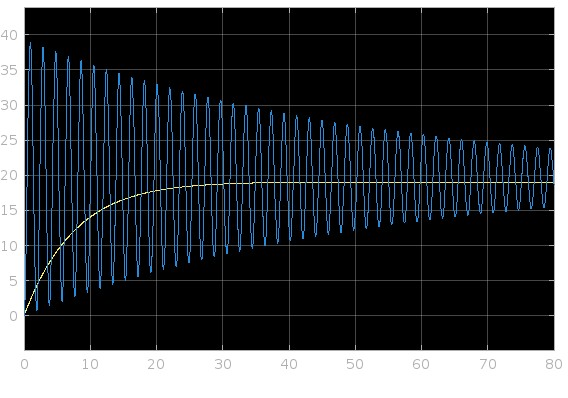
\includegraphics[width=0.6\textwidth]{simulation1.jpg}\par\vspace{1cm}
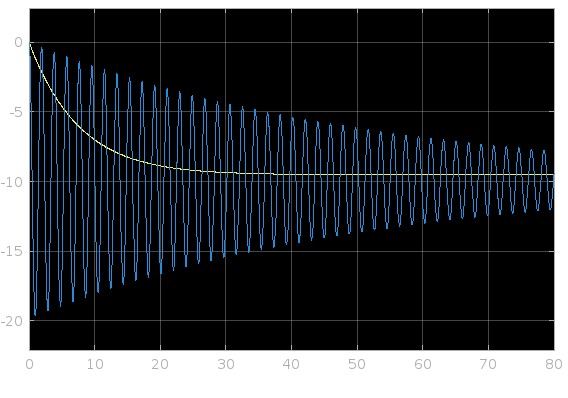
\includegraphics[width=0.6\textwidth]{simulation2.jpg}\par\vspace{1cm}

\section{More complex controller}

(with at least 7 membership functions)

TODO: "Explain and reason what happens if you increase the number of membership functions (7 or more) 
of the output?"

It doesnt talk about it, but if we design the 7 membership functions and the rules, we can implement it in another controller, and run the simulation to see what happens.
I've created pendulum-fuzzy-complex.fis, but so far it is the copy of the original, nothing is modified. 


\section{Conclusions}

%------------------------------------------------------------------------------------------------------------------------------
\section*{References}
\printbibliography[heading=none]

\end{document}